\documentclass{article}
\begin{document}
\subsection{Installation (Linux/MacOS)}
  
\subsubsection{System requirements}

\begin{itemize}
	\item The supported Linux OS versions are Debian based - Ubuntu 18.04 and 22.04.
	\item  The supported macOS versions are MacOS Ventura 13.4.1 and 13.5.2.
\end{itemize} 

\subsubsection{Installation of COINES}
The steps below need to be followed in order to install COINES SDK:
\begin{enumerate}
	\item Download the installer.
	\item Use the command \texttt{cd} to go to the directory where the installer is located and make the installer executable:
	\begin{itemize}
		\item[\$] \texttt{chmod +x coines\_vX.Y.sh}
	\end{itemize}
	\item Ensure that you are connected to the Internet before running the installer, which is executed like this:
	\begin{itemize}
	\item[\$] \texttt{./coines\_vX.Y.sh}
	\end{itemize}	
	\item Accept the End User License agreement
	\begin{figure}[H]
		\begin{center}
			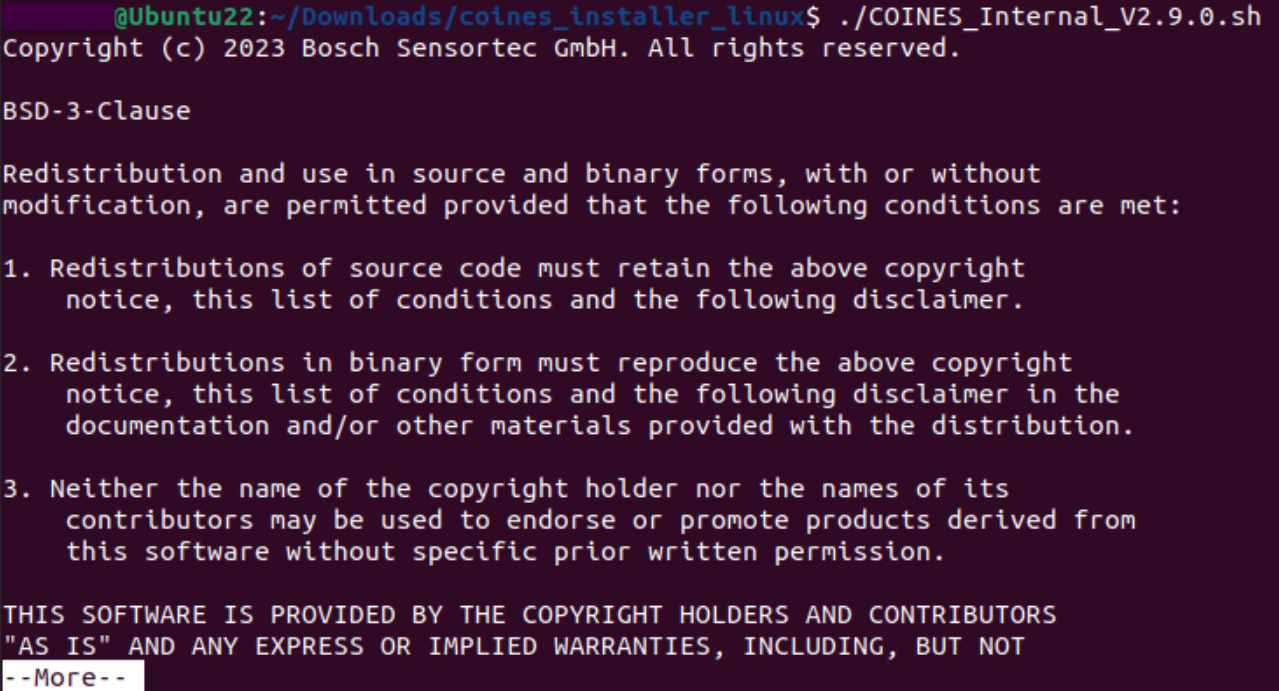
\includegraphics[width=0.7\textwidth]{coinesAPI_images/Linux_installation_user_agreement.png}
		\end{center}
	\end{figure}
	\begin{figure}[H]
		\begin{center}
			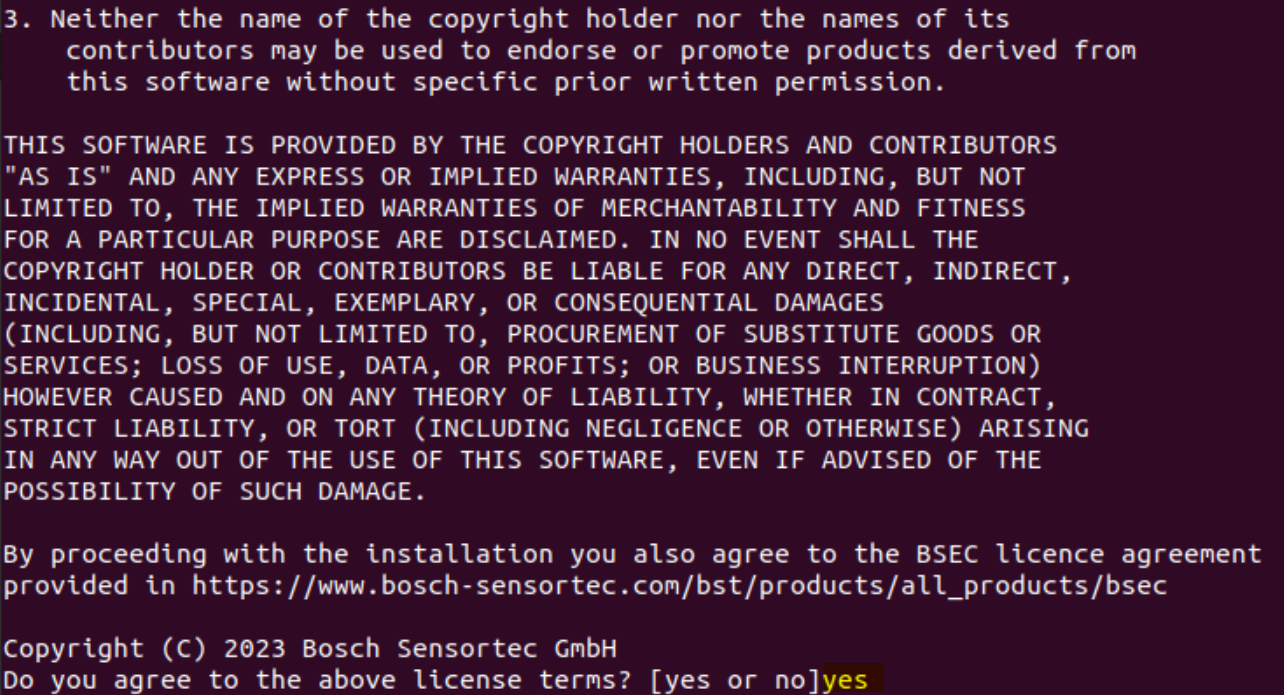
\includegraphics[width=0.7\textwidth]{coinesAPI_images/Linux_installation_user_agreement_1.png}
			\caption{Linux installer end user agreement}
		\end{center}
	\end{figure}
	\item The installer will prompt you if the required dependencies/packages are not installed. (This step requires root privileges.)
\end{enumerate}

\subsubsection{Installation of compiler environment}

On a Debian or Redhat based Linux distro, the installer prompts for installation of missing dependencies, \texttt{gcc}, \texttt{make} and \texttt{libusb-dev} packages.If due to some reason installation fails, the user can manually install the dependencies.
\begin{itemize}
\item Debian based distros - \texttt{gcc}, \texttt{make}, \texttt{libusb-1.0-0-dev}, \texttt{dfu-util} , \texttt{libdbus-1-dev}
\item Redhat based distros - \texttt{gcc}, \texttt{make}, \texttt{libusbx-devel}, \texttt{dfu-util}, \texttt{dbus-devel}
\item MacOS - 
\texttt{libusb}, \texttt{dfu-util}
\end{itemize}

If you intend to run the COINES example on Application Board's microcontroller, download the latest version of \href{https://developer.arm.com/downloads/-/arm-gnu-toolchain-downloads}{GNU Embedded Toolchain for ARM} for Linux and extract the package. Add the compiler to PATH variable by editing \texttt{\$HOME/.bashrc} or similar file like \texttt{/etc/profile or /etc/environment}.


\end{document}